% Chapter Template

\chapter{Results} % Main chapter title

\label{Chapter6} % Change X to a consecutive number; for referencing this chapter elsewhere, use \ref{ChapterX}

\lhead{Chapter 6. \emph{Results}} % Change X to a consecutive number; this is for the header on each page - perhaps a shortened titl

\section{Pentacene}

In this example, we model the dynamics of the pentacene dimer and tetramer using the path integral non-adiabatic dynamics techniques as mentioned.

To study charge transfer processes in molecular aggregates, we use a one-dimensional nearest-neighbours (NN) Hamiltonian of the form [Borelli Ref]. :

\begin{equation} \label{6.x}    
    \mathcal{H} = \sum_{n, m}^{N_e} \epsilon_{nm} \ket{n} \bra{m} + \sum_{k = 1}^{F} \frac{\omega_k}{2} (P_k^{2} + Z_k^{2}) + \sum_{n, k}^{N_e, F} g_k^{(n)} Z_k \ket{n}\bra{n}
\end{equation}

Here $\epsilon_{nm}$ represents the members of a matrix of electronic energies and couplings. For the nearest-neighbour pentacene model we are considering we use a value of $\epsilon_{12} = 300 cm^{-1}$. The "system" part of the Hamiltonian ($\mathcal{H}_s$) is described by the first term of electron couplings. The second term represents the energies of the vibrational modes, treated as harmonic in this case. The third term is the linear coupling between each electron and the vibrational mode at site k. The vibrational frequencies and linear coupling terms are determined by Density Functional Theory calculations [Borelli Hopping Ref]. 

The effects of the bath are taken into consideration by the spectral density. We model the interactions as an effective Debye spectral density with reorganization energy $\lambda = 100 cm^{-1}$ and characteristic frequency $\gamma = 50 cm^{-1}$.

\begin{figure}
    \centering
    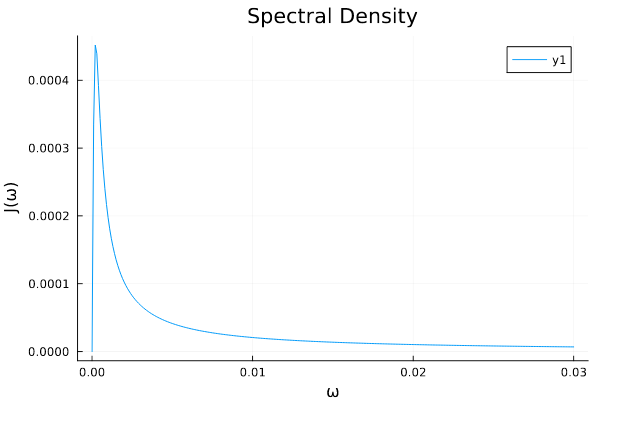
\includegraphics[scale=0.3]{Figures/jw_pentacene.png}
    \caption{Debye Spectral Density for Pentacene}
\end{figure}

Using calculations from the Quantum-Classical Path Integral method, we can see the propagation of the density matrix. We can use this data to obtain the populations of the various sites (diagonal elements) and the coherences between the sites (off-diagonal elements).

\begin{figure}
\centering
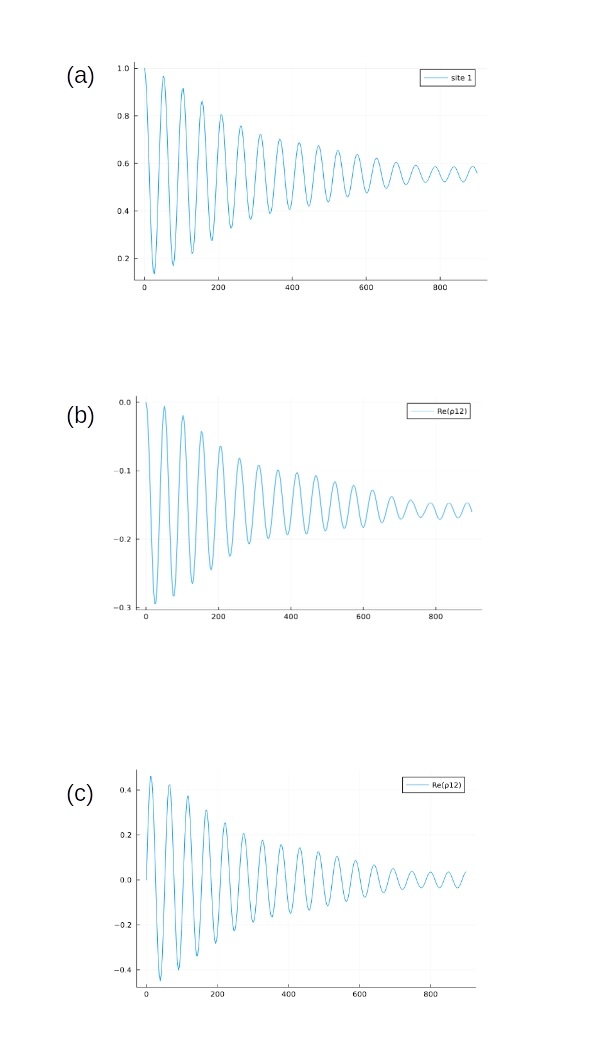
\includegraphics[scale=0.4]{Figures/pentacene_result}
\caption{Density Matrix Elements of Pentacene dimer. (a) $\rho_{11}$ population of site 1 (b) $Re(\rho_{12})$ Real part of coherence (c) $Im(\rho_{12})$ Imaginary part of coherence}
\end{figure}

%\begin{figure}
%\centering
%\includegraphics[scale=0.4]{Figures/pentacene_result2}
%\caption{Density Matrix Elements of Pentacene tetramer. (a) $\rho_{11}$ population of site 1 (b) $Re(\rho_{12})$ Real part of coherence (c) $Im(\rho_{12})$ Imaginary part of coherence}
%\end{figure}



\section{Rubrene}





The effects of the bath are taken into consideration by the spectral density $J(\omega) = \sum_{i} g_i ^{2} \delta(\omega - \omega_i)$. We use a Gaussian line-shape broadening to model the spectral density $J(\omega)$.


\begin{figure}
    \centering
    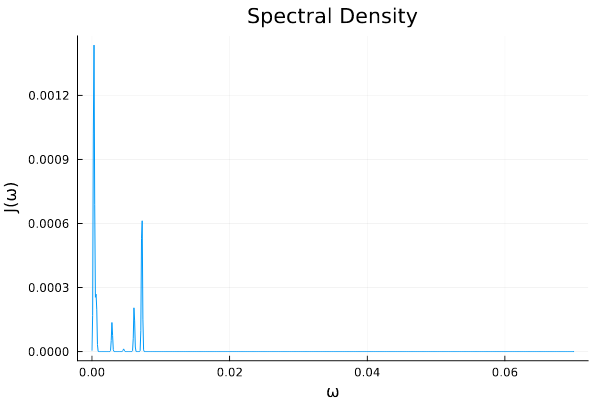
\includegraphics[scale=0.4]{Figures/jw_rubrene.png}
    \caption{Spectral Density (with Gaussian broadening) for Rubrene}
\end{figure}

